\section{Transformada de Fourier}

\begin{frame}[fragile]{Série de Fourier}

    \begin{itemize}
        \item Uma série de Fourier consiste na expansão de uma função períodica $f(x)$ em termos
            de senos e cosenos

        \item Isto possível porque as funções $\sin(mx)$ e $\sin(ny)$ são ortogonais para 
            $m\neq n$ no intervalo $[-\pi, \pi]$:

        \begin{align*}
            \int_{-\pi}^\pi \sin(mx)\sin(nx) dx &= 
            \int_{-\pi}^\pi \sin(mx)\cos(nx) dx \\
            &= \int_{-\pi}^\pi \cos(mx)\cos(nx) dx = 0
        \end{align*}

        \item Para $m = n$, segue que
        \[
            \int_{-\pi}^\pi \sin^2(mx) dx = 
            \int_{-\pi}^\pi \cos^2(mx) dx = \pi
        \]

    \end{itemize}

\end{frame}

\begin{frame}[fragile]{Série de Fourier}

    \begin{itemize}
        \item Deste modo,
        \[
            f(x) = \frac{1}{2}a_0 + \sum_{n=1}^\infty a_n\cos(n x) + \sum_{n=1}^\infty b_n\sin(nx),
        \]
        onde
        \begin{align*}
            a_0 &= \frac{1}{\pi}\int_{-\pi}^{\pi} f(x)dx \\    
            a_n &= \frac{1}{\pi}\int_{-\pi}^{\pi} f(x)\cos(nx)dx \\    
            b_n &= \frac{1}{\pi}\int_{-\pi}^{\pi} f(x)\sin(nx)dx    
        \end{align*}
    
    \end{itemize}

\end{frame}

\begin{frame}[fragile]{Exemplo: Onda Quadrada}

    Considere a onda quadrada abaixo:

    \begin{figure}
        \centering

        \begin{tikzpicture}
            \draw[very thick] (-1, 0) -- (0, 0) -- (0, 2) -- (pi, 2) -- (pi, 0) -- ({2*pi}, 0)
                -- (2*pi, 2) -- (3*pi, 2) -- (3*pi, 0) -- (10, 0);

            \node[anchor=east] at (0, 2) { $a$ };
            \node[anchor=north] at (pi, 0) { $\pi$ };
            \node[anchor=north] at (2*pi, 0) { $2\pi$ };
            \node[anchor=north] at (3*pi, 0) { $3\pi$ };

%            \draw[blue!60!black,domain=-1:10,samples=201] plot (\x, {1 + (4/pi)*sin(\x*180/pi)
%               + (4/(3*pi))*sin(\x*3*180/pi)
%                + (4/(5*pi))*sin(\x*5*180/pi)
%                + (4/(7*pi))*sin(\x*7*180/pi)
%});

            \draw[->] (0,-1) -- (0, 3.2) node[anchor=east] { $x$ };
            \draw[->] (-1,0) -- (10.2, 0) node[anchor=north] { $t$ };
        \end{tikzpicture}
    \end{figure}

\end{frame}

\begin{frame}[fragile]{Exemplo: Onda Quadrada}

    \begin{itemize}
        \item O coeficiente $a_0$ é dado por
        \[
            a_0 = \frac{1}{\pi}\int_{-\pi}^{\pi} f(t)dt = \frac{1}{\pi}\int_{0}^{\pi} a\, dt = a
        \]

        \item Os coeficientes $a_n$, para $n\geq 1$, são todos iguais a zero, pois
        \[
            a_n = \frac{1}{\pi}\int_{-\pi}^{\pi} f(t)\cos(nt) dt 
                = \frac{a}{\pi}\left[\left.\frac{\sin(nt)}{n}\right\rvert_0^\pi\right] = 0
        \]

        \item Os coeficientes $b_n$ são iguais a zero, para $n$ par, e
        \[
            b_n = \frac{1}{\pi}\int_{-\pi}^{\pi} f(t)\sin(nt) dt 
                = -\frac{a}{\pi}\left[\left.\frac{\cos(nt)}{n}\right\rvert_0^\pi\right] = \frac{2a}{m\pi},
        \]
        se $n$ é ímpar
    \end{itemize}

\end{frame}

\begin{frame}[fragile]{Exemplo: Aproximação da onda quadrada com $n = 0$}

    \begin{figure}
        \centering

        \begin{tikzpicture}
            \draw[very thick] (-1, 0) -- (0, 0) -- (0, 2) -- (pi, 2) -- (pi, 0) -- ({2*pi}, 0)
                -- (2*pi, 2) -- (3*pi, 2) -- (3*pi, 0) -- (10, 0);

            \node[anchor=east] at (0, 2) { $a$ };
            \node[anchor=north] at (pi, 0) { $\pi$ };
            \node[anchor=north] at (2*pi, 0) { $2\pi$ };
            \node[anchor=north] at (3*pi, 0) { $3\pi$ };

            \draw[blue!60!black,domain=-1:10,samples=201] plot (\x, {1 
% + (4/pi)*sin(\x*180/pi)
%               + (4/(3*pi))*sin(\x*3*180/pi)
%                + (4/(5*pi))*sin(\x*5*180/pi)
%                + (4/(7*pi))*sin(\x*7*180/pi)
});

            \draw[->] (0,-1) -- (0, 3.2) node[anchor=east] { $x$ };
            \draw[->] (-1,0) -- (10.2, 0) node[anchor=north] { $t$ };
        \end{tikzpicture}
    \end{figure}

\end{frame}

\begin{frame}[fragile]{Exemplo: Aproximação da onda quadrada com $n = 1$}

    \begin{figure}
        \centering

        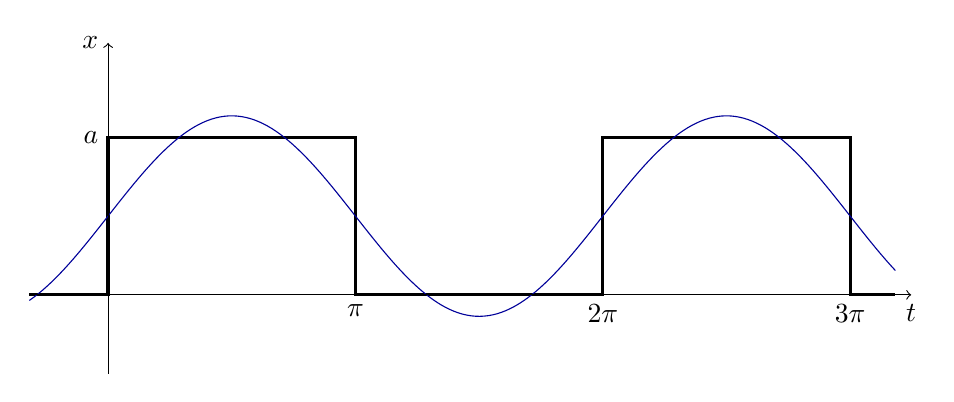
\begin{tikzpicture}
            \draw[very thick] (-1, 0) -- (0, 0) -- (0, 2) -- (pi, 2) -- (pi, 0) -- ({2*pi}, 0)
                -- (2*pi, 2) -- (3*pi, 2) -- (3*pi, 0) -- (10, 0);

            \node[anchor=east] at (0, 2) { $a$ };
            \node[anchor=north] at (pi, 0) { $\pi$ };
            \node[anchor=north] at (2*pi, 0) { $2\pi$ };
            \node[anchor=north] at (3*pi, 0) { $3\pi$ };

            \draw[blue!60!black,domain=-1:10,samples=201] plot (\x, {1 
                + (4/pi)*sin(\x*180/pi)
%               + (4/(3*pi))*sin(\x*3*180/pi)
%               + (4/(5*pi))*sin(\x*5*180/pi)
%               + (4/(7*pi))*sin(\x*7*180/pi)
});

            \draw[->] (0,-1) -- (0, 3.2) node[anchor=east] { $x$ };
            \draw[->] (-1,0) -- (10.2, 0) node[anchor=north] { $t$ };
        \end{tikzpicture}
    \end{figure}

\end{frame}

\begin{frame}[fragile]{Exemplo: Aproximação da onda quadrada com $n = 3$}

    \begin{figure}
        \centering

        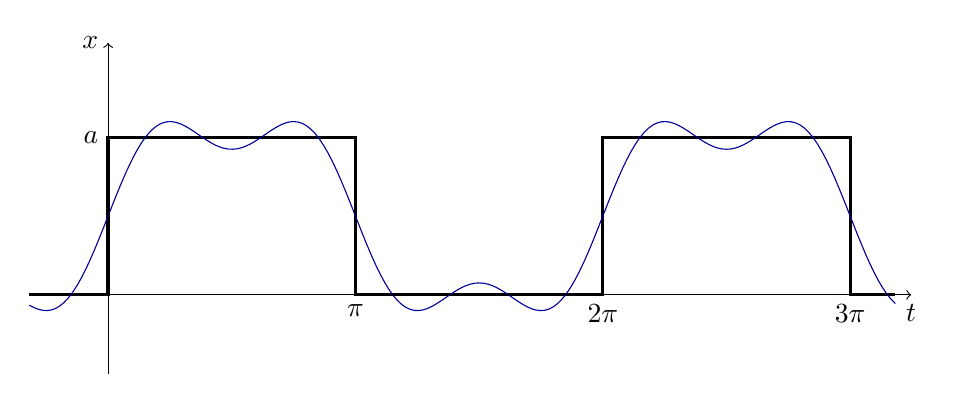
\begin{tikzpicture}
            \draw[very thick] (-1, 0) -- (0, 0) -- (0, 2) -- (pi, 2) -- (pi, 0) -- ({2*pi}, 0)
                -- (2*pi, 2) -- (3*pi, 2) -- (3*pi, 0) -- (10, 0);

            \node[anchor=east] at (0, 2) { $a$ };
            \node[anchor=north] at (pi, 0) { $\pi$ };
            \node[anchor=north] at (2*pi, 0) { $2\pi$ };
            \node[anchor=north] at (3*pi, 0) { $3\pi$ };

            \draw[blue!60!black,domain=-1:10,samples=201] plot (\x, {1 
                + (4/pi)*sin(\x*180/pi)
               + (4/(3*pi))*sin(\x*3*180/pi)
%               + (4/(5*pi))*sin(\x*5*180/pi)
%               + (4/(7*pi))*sin(\x*7*180/pi)
});

            \draw[->] (0,-1) -- (0, 3.2) node[anchor=east] { $x$ };
            \draw[->] (-1,0) -- (10.2, 0) node[anchor=north] { $t$ };
        \end{tikzpicture}
    \end{figure}

\end{frame}

\begin{frame}[fragile]{Exemplo: Aproximação da onda quadrada com $n = 5$}

    \begin{figure}
        \centering

        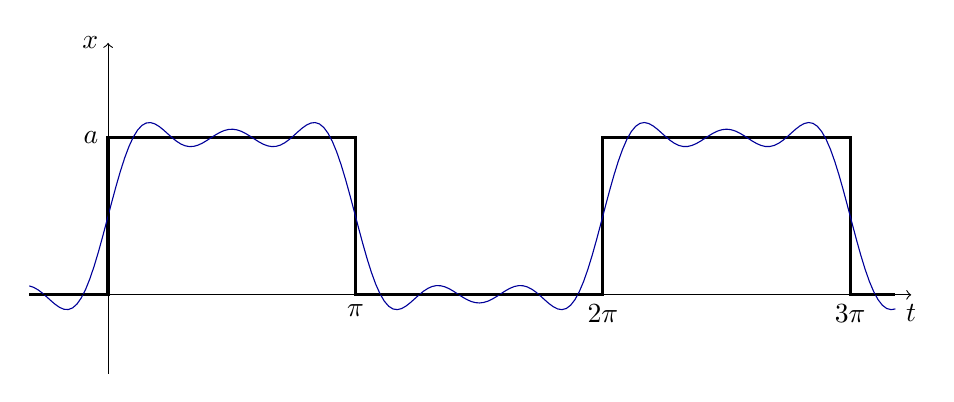
\begin{tikzpicture}
            \draw[very thick] (-1, 0) -- (0, 0) -- (0, 2) -- (pi, 2) -- (pi, 0) -- ({2*pi}, 0)
                -- (2*pi, 2) -- (3*pi, 2) -- (3*pi, 0) -- (10, 0);

            \node[anchor=east] at (0, 2) { $a$ };
            \node[anchor=north] at (pi, 0) { $\pi$ };
            \node[anchor=north] at (2*pi, 0) { $2\pi$ };
            \node[anchor=north] at (3*pi, 0) { $3\pi$ };

            \draw[blue!60!black,domain=-1:10,samples=201] plot (\x, {1 
                + (4/pi)*sin(\x*180/pi)
               + (4/(3*pi))*sin(\x*3*180/pi)
               + (4/(5*pi))*sin(\x*5*180/pi)
%               + (4/(7*pi))*sin(\x*7*180/pi)
});

            \draw[->] (0,-1) -- (0, 3.2) node[anchor=east] { $x$ };
            \draw[->] (-1,0) -- (10.2, 0) node[anchor=north] { $t$ };
        \end{tikzpicture}
    \end{figure}

\end{frame}

\begin{frame}[fragile]{Exemplo: Aproximação da onda quadrada com $n = 7$}

    \begin{figure}
        \centering

        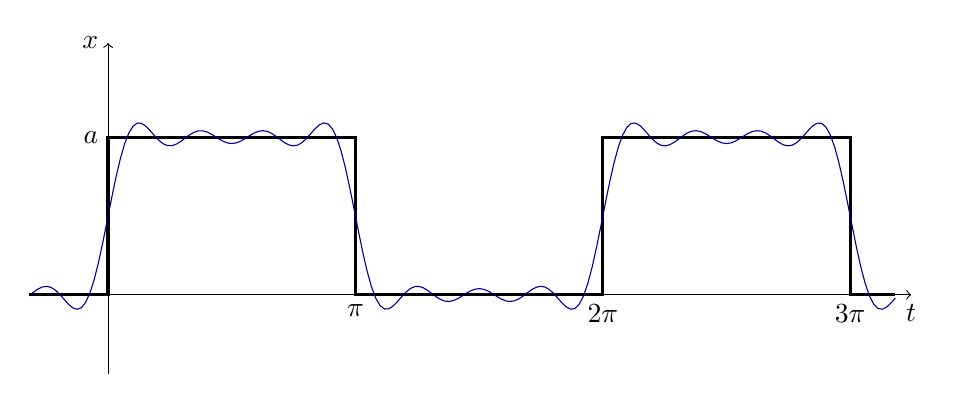
\begin{tikzpicture}
            \draw[very thick] (-1, 0) -- (0, 0) -- (0, 2) -- (pi, 2) -- (pi, 0) -- ({2*pi}, 0)
                -- (2*pi, 2) -- (3*pi, 2) -- (3*pi, 0) -- (10, 0);

            \node[anchor=east] at (0, 2) { $a$ };
            \node[anchor=north] at (pi, 0) { $\pi$ };
            \node[anchor=north] at (2*pi, 0) { $2\pi$ };
            \node[anchor=north] at (3*pi, 0) { $3\pi$ };

            \draw[blue!60!black,domain=-1:10,samples=201] plot (\x, {1 
                + (4/pi)*sin(\x*180/pi)
               + (4/(3*pi))*sin(\x*3*180/pi)
               + (4/(5*pi))*sin(\x*5*180/pi)
               + (4/(7*pi))*sin(\x*7*180/pi)
});

            \draw[->] (0,-1) -- (0, 3.2) node[anchor=east] { $x$ };
            \draw[->] (-1,0) -- (10.2, 0) node[anchor=north] { $t$ };
        \end{tikzpicture}
    \end{figure}

\end{frame}

\begin{frame}[fragile]{Série de Fourier com coeficientes complexos}

    \begin{itemize}
        \item A série de Fourier pode ser estendida para coeficientes complexos a partir da
            observação que
        \[
            e^{bi} = \cos b + i\sin b
        \]

        \item Seja $f(x)$ uma função nos reais. Faça
        \[
            f(x) = \sum_{-\infty}^\infty A_ne^{inx}
        \]

        \item Assim, vale que
        \[
            \int_{-\pi}^\pi f(x)e^{-imx}dx = 2\pi A_m,
        \]
        de modo que
        \[
            A_n = \frac{1}{2\pi}\int_{-\pi}^{\pi} f(x)e^{-in x}dx
        \]
    \end{itemize}

\end{frame}

\begin{frame}[fragile]{Exemplo: Onda Triangular}

    Considere a onda triangular abaixo:

    \begin{figure}
        \centering

        \begin{tikzpicture}
            \draw[very thick] (-1, 1) -- (0, 0) -- (pi, pi) -- (2*pi, 0) -- (3*pi, pi) -- (10, 2.566);

            \node[anchor=east] at (0, pi) { $\pi$ };
            \node[anchor=north] at (pi, 0) { $\pi$ };
            \node[anchor=north] at (2*pi, 0) { $2\pi$ };
            \node[anchor=north] at (3*pi, 0) { $3\pi$ };

%            \draw[blue!60!black,domain=-1:10,samples=201] plot (\x, {pi*(1/2) 
%                - (1/(2)*(4)*cos(\x*180/pi)
%               - (1/(2))*(4/9)*cos(\x*3*180/pi)
%               - (1/(2))*(4/25)*cos(\x*5*180/pi)
%               - (1/(2))*(4/49)*cos(\x*7*180/pi)
%               - (1/(2))*(4/81)*cos(\x*9*180/pi)
%});

            \draw[->] (0,-1) -- (0, 4.2) node[anchor=east] { $x$ };
            \draw[->] (-1,0) -- (10.2, 0) node[anchor=north] { $t$ };
        \end{tikzpicture}
    \end{figure}

\end{frame}

\begin{frame}[fragile]{Exemplo: Onda Triangular}

    \begin{itemize}
        \item No intervalo $[-\pi, \pi]$ temos que
        \[
            f(x) = \left\{ \begin{array}{cc}
                                -x,& \mbox{se}\ x \leq 0,\\
                                x,& \mbox{caso contrário}
                           \end{array}\right.
        \]

        \item Daí
        \[
            A_0 = \frac{1}{2\pi}\int_{-\pi}^\pi f(x)dx = \frac{\pi}{2}
        \]

        \item Para $n > 1$ ímpar vale que
        \[
            A_n = \frac{1}{2\pi}\int_{-\pi}^\pi f(x)e^{inx}dx = -\frac{4}{n^2}
        \]
        
        \item $A_n = 0$, se $n$ é par
    \end{itemize}

\end{frame}

\begin{frame}[fragile]{Exemplo: Aproximação com $n = 0$}

    \begin{figure}
        \centering

        \begin{tikzpicture}
            \draw[very thick] (-1, 1) -- (0, 0) -- (pi, pi) -- (2*pi, 0) -- (3*pi, pi) -- (10, 2.566);

            \node[anchor=east] at (0, pi) { $\pi$ };
            \node[anchor=north] at (pi, 0) { $\pi$ };
            \node[anchor=north] at (2*pi, 0) { $2\pi$ };
            \node[anchor=north] at (3*pi, 0) { $3\pi$ };

            \draw[blue!60!black,domain=-1:10,samples=201] plot (\x, {pi*(1/2) 
%                - (1/(2)*(4)*cos(\x*180/pi)
%               - (1/(2))*(4/9)*cos(\x*3*180/pi)
%               - (1/(2))*(4/25)*cos(\x*5*180/pi)
%               - (1/(2))*(4/49)*cos(\x*7*180/pi)
%               - (1/(2))*(4/81)*cos(\x*9*180/pi)
});

            \draw[->] (0,-1) -- (0, 4.2) node[anchor=east] { $x$ };
            \draw[->] (-1,0) -- (10.2, 0) node[anchor=north] { $t$ };
        \end{tikzpicture}
    \end{figure}

\end{frame}

\begin{frame}[fragile]{Exemplo: Aproximação com $n = 1$}

    \begin{figure}
        \centering

        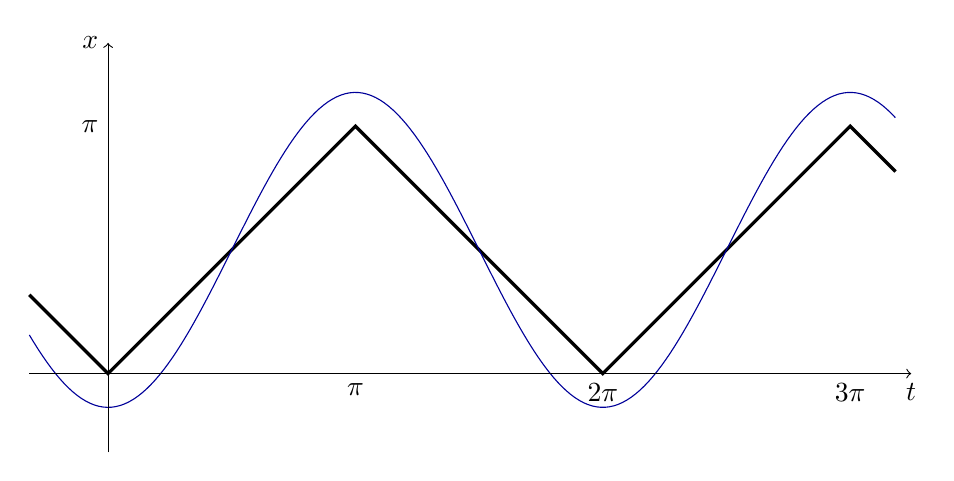
\begin{tikzpicture}
            \draw[very thick] (-1, 1) -- (0, 0) -- (pi, pi) -- (2*pi, 0) -- (3*pi, pi) -- (10, 2.566);

            \node[anchor=east] at (0, pi) { $\pi$ };
            \node[anchor=north] at (pi, 0) { $\pi$ };
            \node[anchor=north] at (2*pi, 0) { $2\pi$ };
            \node[anchor=north] at (3*pi, 0) { $3\pi$ };

            \draw[blue!60!black,domain=-1:10,samples=201] plot (\x, {pi*(1/2) 
                - (1/(2)*(4)*cos(\x*180/pi)
%               - (1/(2))*(4/9)*cos(\x*3*180/pi)
%               - (1/(2))*(4/25)*cos(\x*5*180/pi)
%               - (1/(2))*(4/49)*cos(\x*7*180/pi)
%               - (1/(2))*(4/81)*cos(\x*9*180/pi)
});

            \draw[->] (0,-1) -- (0, 4.2) node[anchor=east] { $x$ };
            \draw[->] (-1,0) -- (10.2, 0) node[anchor=north] { $t$ };
        \end{tikzpicture}
    \end{figure}

\end{frame}

\begin{frame}[fragile]{Exemplo: Aproximação com $n = 3$}

    \begin{figure}
        \centering

        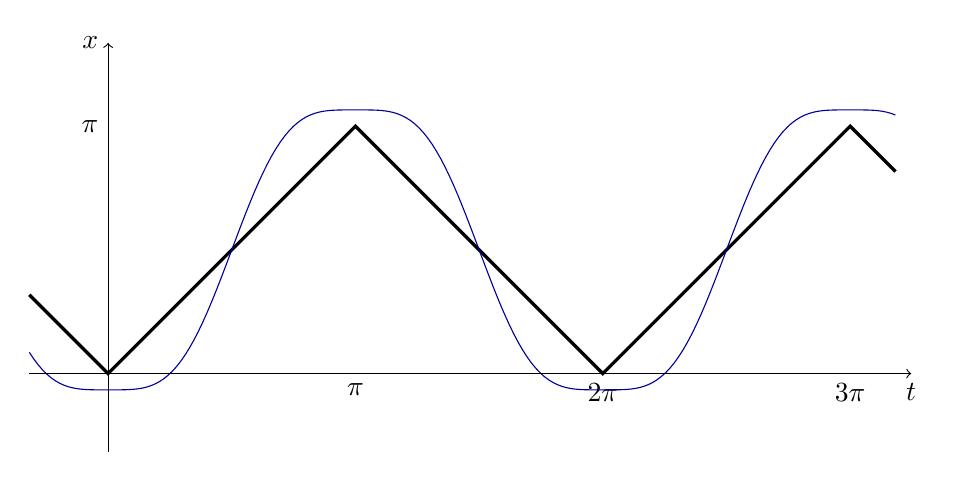
\begin{tikzpicture}
            \draw[very thick] (-1, 1) -- (0, 0) -- (pi, pi) -- (2*pi, 0) -- (3*pi, pi) -- (10, 2.566);

            \node[anchor=east] at (0, pi) { $\pi$ };
            \node[anchor=north] at (pi, 0) { $\pi$ };
            \node[anchor=north] at (2*pi, 0) { $2\pi$ };
            \node[anchor=north] at (3*pi, 0) { $3\pi$ };

            \draw[blue!60!black,domain=-1:10,samples=201] plot (\x, {pi*(1/2) 
                - (1/(2)*(4)*cos(\x*180/pi)
               - (1/(2))*(4/9)*cos(\x*3*180/pi)
%               - (1/(2))*(4/25)*cos(\x*5*180/pi)
%               - (1/(2))*(4/49)*cos(\x*7*180/pi)
%               - (1/(2))*(4/81)*cos(\x*9*180/pi)
});

            \draw[->] (0,-1) -- (0, 4.2) node[anchor=east] { $x$ };
            \draw[->] (-1,0) -- (10.2, 0) node[anchor=north] { $t$ };
        \end{tikzpicture}
    \end{figure}

\end{frame}

\begin{frame}[fragile]{Exemplo: Aproximação com $n = 5$}

    \begin{figure}
        \centering

        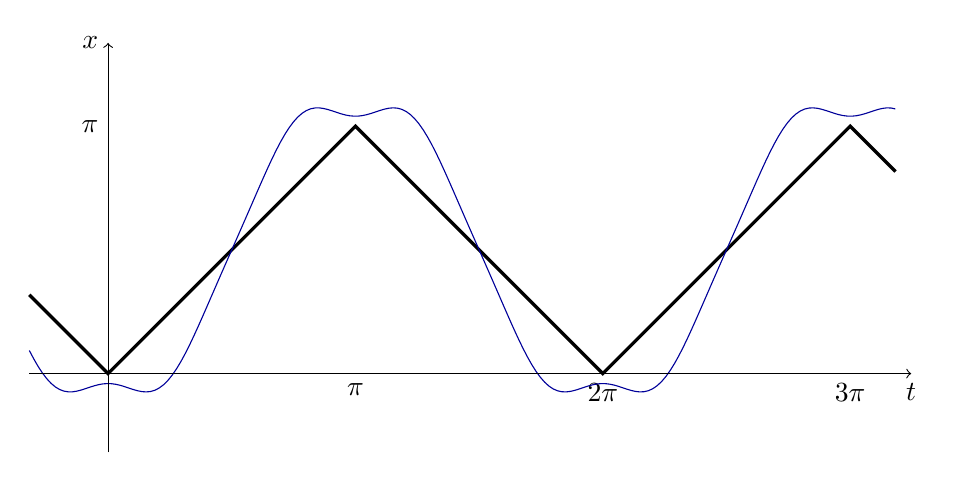
\begin{tikzpicture}
            \draw[very thick] (-1, 1) -- (0, 0) -- (pi, pi) -- (2*pi, 0) -- (3*pi, pi) -- (10, 2.566);

            \node[anchor=east] at (0, pi) { $\pi$ };
            \node[anchor=north] at (pi, 0) { $\pi$ };
            \node[anchor=north] at (2*pi, 0) { $2\pi$ };
            \node[anchor=north] at (3*pi, 0) { $3\pi$ };

            \draw[blue!60!black,domain=-1:10,samples=201] plot (\x, {pi*(1/2) 
                - (1/(2)*(4)*cos(\x*180/pi)
               - (1/(2))*(4/9)*cos(\x*3*180/pi)
               - (1/(2))*(4/25)*cos(\x*5*180/pi)
%               - (1/(2))*(4/49)*cos(\x*7*180/pi)
%               - (1/(2))*(4/81)*cos(\x*9*180/pi)
});

            \draw[->] (0,-1) -- (0, 4.2) node[anchor=east] { $x$ };
            \draw[->] (-1,0) -- (10.2, 0) node[anchor=north] { $t$ };
        \end{tikzpicture}
    \end{figure}

\end{frame}

\begin{frame}[fragile]{Transformada de Fourier}

    \begin{itemize}
        \item A transformada de Fourier é uma generalização das séries de Fourier com coeficientes
            complexos quando o período tende ao infinito

        \item Seja $f(x)$ uma função com um número finito de descontinuidades e tal existe a
        integral
        \[
            \int_{-\infty}^\infty |f(x)|dx
        \]

        \item A Transformada de Fourier $\mathcal{F}$ de $f(x)$ é dada por
        \[
            \mathcal{F}[f(x)] = F(k) = \int_{-\infty}^{\infty} f(x)e^{-2\pi ikx} dx
        \]
         
        \item A Transformada Inversa $\mathcal{F}^{-1}$ é dada por
        \[
            \mathcal{F}^{-1}[F(k)] = f(x) = \int_{-\infty}^{\infty} F(k)e^{2\pi ikx} dk
        \]

    \end{itemize}

\end{frame}

\begin{frame}[fragile]{Propriedades}

    \begin{itemize}
        \item A Transformada de Fourier é linear:
        \[
            \mathcal{F}[af(x) + bg(x)] = a\mathcal{F}[f(x)] + b\mathcal{F}[g(x)],
        \]
        onde $a$ e $b$ são constantes

        \item A transformada da derivada da função está diretamente relacionada com a transformada
            da função
        \[
            \mathcal{F}[f^{(n)}(x)](k) = (2\pi ik)^n\mathcal{F}[f(x)](k)
        \]

        \item \textbf{Teorema da Convolução}:
        \[
            \mathcal{F}[f*g] = \mathcal{F}[f]\mathcal{F}[g]
        \]
    \end{itemize}

\end{frame}

\begin{frame}[fragile]{Exemplo: Exponencial Descrescente}

    \begin{itemize}
        \item Seja
        \[
            f(x) = \left\{ \begin{array}{cc}
                                e^{-x},& \mbox{se}\ x \geq 0,\\
                                0,& \mbox{caso contrário}
                        \end{array}\right.
        \]

        \item Temos que
        \begin{align*}
            \mathcal{F}[f(x)] = F(k) &= \int_{-\infty}^\infty f(x)e^{-2\pi ikx}dx \\
            &= \int_0^\infty e^{-x}e^{-2\pi ikx}dx = \int_0^\infty e^{-(1 + 2\pi ik)x}dx \\
            &= \left. -\frac{e^{-(1 + 2\pi ik)x}}{1 + 2\pi ik}\right|_0^\infty\\
            &= \frac{1}{1 + 2\pi ik}
        \end{align*}
    \end{itemize}

\end{frame}

\begin{frame}[fragile]{Visualização da função $f(x)$}

    \begin{figure}
        \centering

        \begin{tikzpicture}
            \node[anchor=east] at (0, 5) { \tt \small 1 };

            \draw[thick,blue,domain=0:10,samples=201] plot (\x, { 5*exp(-\x) });
%            \draw[blue!60!black,domain=0:5,samples=201] plot (\x + 6, { 1/(1 + 2*pi*\x) });

            \draw[->] (0,-1) -- (0, 5.7) node[anchor=east] { $f(x)$ };
            \draw[->] (-1,0) -- (10.2, 0) node[anchor=north] { $x$ };

        \end{tikzpicture}
    \end{figure}

\end{frame}

\begin{frame}[fragile]{Visualização da parte real (azul) e imaginária (vermelha) da função $F(k)$}

    \begin{figure}
        \centering

        \begin{tikzpicture}
            \node[anchor=east] at (0, 3) { \tt \footnotesize 1 };
            \node[anchor=east] at (0, -3) { \tt \footnotesize -1 };
            \node[anchor=north] at (3, 0) { \tt \footnotesize 1 };
            \node[anchor=north] at (-3, 0) { \tt \footnotesize -1 };

            \draw[blue!80!black,domain=-1.1:1.1,samples=201] plot (\x*3, { 3/(1 + 4*pi*pi*\x*\x) });
            \draw[red!90!black,domain=-1.1:1.1,samples=201] plot (\x*3, { (-3*2*pi*\x)/(1 + 4*pi*pi*\x*\x) });

            \draw[->] (0,-3.2) -- (0, 3.8) node[anchor=east] { $F(k)$ };
            \draw[->] (-3.8,0) -- (3.8, 0) node[anchor=north] { $k$ };

        \end{tikzpicture}
    \end{figure}

\end{frame}

\begin{frame}[fragile]{Transformada Discreta de Fourier}

    \begin{itemize}
        \item Uma série $x_i = \{ x_0, x_1, \ldots, x_{N - 1}$ de $N$ amostras de um sinal,
            igualmente espaçadas ao longo do tempo,
            pode ser interpretada como uma função $y_i$ períodica de período $N$

        \item Para isso, defina $y(j) = x_i$, onde $j$ é um inteiro tal que $j = N*q + i$, e
            $y(t) = 0$, se $t$ não é inteiro

        \item Contudo, ao invés de fazer esta adaptação e utilizar a transformada de Fourier, é
            melhor utilizar a Transformada Discreta de Fourier (DFT):
        \[
            X_k = \sum_{n = 0}^{N - 1} x_ne^{-2\pi ikn/N}
        \]

        \item A Transformada Discreta Inversa de Fourier (IDFT) é dada por:
        \[
            x_n = \frac{1}{N}\sum_{k = 0}^{N - 1} F_ke^{2\pi ikn/N}
        \]

    \end{itemize}

\end{frame}

\begin{frame}[fragile]{Implementação da DFT e da IDFT em C++ em $O(N^2)$}
    \inputsnippet{cpp}{1}{20}{codes/dft.cpp}
\end{frame}

\begin{frame}[fragile]{Implementação da DFT e da IDFT em C++ em $O(N^2)$}
    \inputsnippet{cpp}{21}{32}{codes/dft.cpp}
\end{frame}

\begin{frame}[fragile]{Aplicação da DFT: Multiplicação de Polinômios}

    \begin{itemize}
        \item A convolução entre duas funções $f(x)$ e $g(x)$ é uma função $h(x) = f(x)*g(x)$
            que representa como a forma de uma função é modificada pela outra

        \item Ela é a integral do produto de ambas funções, sendo que uma delas é invertida e
            deslocada:
        \[
            h(x) = f(x)*g(x) = \int_{-\infty}^\infty f(\tau)(t - \tau)\, d\tau
        \]

        \item A convolução discreta de $f$ e $g$ é dada por
        \[
            (f * g)[n] = \sum_{m=-\infty}^\infty f[m]g[n - m]
        \]

        \item Se $f(x)$ e $g(x)$ são sequências de coeficientes de dois polinômios, a convolução
            de ambas será igual ao produto destes polinômios
    \end{itemize}

\end{frame}

\begin{frame}[fragile]{Visualização da multiplicação de polinômios}

    \begin{figure}
        \centering

        \begin{tikzpicture}
            \node[anchor=west] at (0, 7) { $f(x) = x^2 - 5x + 6$ };
            \node[anchor=west] at (0, 6.5) { $g(x) = x^3 - 2x^2 + 3x - 1$ };
            \node[opacity=0,anchor=west] at (0, 6) { $h(x) = $};

            \draw[opacity=0] (1, 2) grid (10, 3);
            \draw (4, 2) grid (8, 3);
            \draw (4, 3) grid (7, 4);

            \node at (4.5, 3.5) { \tt 6 };
            \node at (5.5, 3.5) { \tt -5 };
            \node at (6.5, 3.5) { \tt 1 };

            \node at (4.5, 2.5) { \tt -1 };
            \node at (5.5, 2.5) { \tt 3 };
            \node at (6.5, 2.5) { \tt -2 };
            \node at (7.5, 2.5) { \tt 1 };
        \end{tikzpicture}

    \end{figure}

\end{frame}

\begin{frame}[fragile]{Visualização da multiplicação de polinômios}

    \begin{figure}
        \centering

        \begin{tikzpicture}
            \node[anchor=west] at (0, 7) { $f(x) = x^2 - 5x + 6$ };
            \node[anchor=west] at (0, 6.5) { $g(x) = x^3 - 2x^2 + 3x - 1$ };
            \node[anchor=west] at (0, 6) { $h(x) = \mathbf{-6}$};

            \draw[opacity=0] (1, 2) grid (10, 3);
            \draw (1, 2) grid (5, 3);
            \draw (4, 3) grid (7, 4);

            \node at (4.5, 3.5) { \tt \textcolor{blue}{6} };
            \node at (5.5, 3.5) { \tt -5 };
            \node at (6.5, 3.5) { \tt 1 };

            \node at (4.5, 2.5) { \tt \textcolor{blue}{-1} };
            \node at (3.5, 2.5) { \tt 3 };
            \node at (2.5, 2.5) { \tt -2 };
            \node at (1.5, 2.5) { \tt 1 };
        \end{tikzpicture}

    \end{figure}

\end{frame}

\begin{frame}[fragile]{Visualização da multiplicação de polinômios}

    \begin{figure}
        \centering

        \begin{tikzpicture}
            \node[anchor=west] at (0, 7) { $f(x) = x^2 - 5x + 6$ };
            \node[anchor=west] at (0, 6.5) { $g(x) = x^3 - 2x^2 + 3x - 1$ };
            \node[anchor=west] at (0, 6) { $h(x) = \mathbf{23}x - 6$};

            \draw[opacity=0] (1, 2) grid (10, 3);
            \draw (2, 2) grid (6, 3);
            \draw (4, 3) grid (7, 4);

            \node at (4.5, 3.5) { \tt \textcolor{blue}{6} };
            \node at (5.5, 3.5) { \tt \textcolor{red}{-5} };
            \node at (6.5, 3.5) { \tt 1 };

            \node at (5.5, 2.5) { \tt \textcolor{red}{-1} };
            \node at (4.5, 2.5) { \tt \textcolor{blue}{3} };
            \node at (3.5, 2.5) { \tt -2 };
            \node at (2.5, 2.5) { \tt 1 };
        \end{tikzpicture}

    \end{figure}

\end{frame}

\begin{frame}[fragile]{Visualização da multiplicação de polinômios}

    \begin{figure}
        \centering

        \begin{tikzpicture}
            \node[anchor=west] at (0, 7) { $f(x) = x^2 - 5x + 6$ };
            \node[anchor=west] at (0, 6.5) { $g(x) = x^3 - 2x^2 + 3x - 1$ };
            \node[anchor=west] at (0, 6) { $h(x) = \mathbf{-28}x^2 + 23x - 6$};

            \draw[opacity=0] (1, 2) grid (10, 3);
            \draw (3, 2) grid (7, 3);
            \draw (4, 3) grid (7, 4);

            \node at (4.5, 3.5) { \tt \textcolor{blue}{6} };
            \node at (5.5, 3.5) { \tt \textcolor{red}{-5} };
            \node at (6.5, 3.5) { \tt \textcolor{green!60!black}{1} };

            \node at (6.5, 2.5) { \tt \textcolor{green!60!black}{-1} };
            \node at (5.5, 2.5) { \tt \textcolor{red}{3} };
            \node at (4.5, 2.5) { \tt \textcolor{blue}{-2} };
            \node at (3.5, 2.5) { \tt 1 };
        \end{tikzpicture}

    \end{figure}

\end{frame}

\begin{frame}[fragile]{Visualização da multiplicação de polinômios}

    \begin{figure}
        \centering

        \begin{tikzpicture}
            \node[anchor=west] at (0, 7) { $f(x) = x^2 - 5x + 6$ };
            \node[anchor=west] at (0, 6.5) { $g(x) = x^3 - 2x^2 + 3x - 1$ };
            \node[anchor=west] at (0, 6) { $h(x) = \mathbf{19}x^3 - 28x^2 + 23x - 6$};

            \draw[opacity=0] (1, 2) grid (10, 3);
            \draw (4, 2) grid (8, 3);
            \draw (4, 3) grid (7, 4);

            \node at (4.5, 3.5) { \tt \textcolor{blue}{6} };
            \node at (5.5, 3.5) { \tt \textcolor{red}{-5} };
            \node at (6.5, 3.5) { \tt \textcolor{green!60!black}{1} };

            \node at (7.5, 2.5) { \tt \textcolor{black}{-1} };
            \node at (6.5, 2.5) { \tt \textcolor{green!60!black}{3} };
            \node at (5.5, 2.5) { \tt \textcolor{red}{-2} };
            \node at (4.5, 2.5) { \tt \textcolor{blue}{1} };
        \end{tikzpicture}

    \end{figure}

\end{frame}

\begin{frame}[fragile]{Visualização da multiplicação de polinômios}

    \begin{figure}
        \centering

        \begin{tikzpicture}
            \node[anchor=west] at (0, 7) { $f(x) = x^2 - 5x + 6$ };
            \node[anchor=west] at (0, 6.5) { $g(x) = x^3 - 2x^2 + 3x - 1$ };
            \node[anchor=west] at (0, 6) { $h(x) = \mathbf{-7}x^4 + 19x^3 - 28x^2 + 23x - 6$};

            \draw[opacity=0] (1, 2) grid (10, 3);
            \draw (5, 2) grid (9, 3);
            \draw (4, 3) grid (7, 4);

            \node at (4.5, 3.5) { \tt \textcolor{black}{6} };
            \node at (5.5, 3.5) { \tt \textcolor{red}{-5} };
            \node at (6.5, 3.5) { \tt \textcolor{green!60!black}{1} };

            \node at (8.5, 2.5) { \tt \textcolor{black}{-1} };
            \node at (7.5, 2.5) { \tt \textcolor{black}{3} };
            \node at (6.5, 2.5) { \tt \textcolor{green!60!black}{-2} };
            \node at (5.5, 2.5) { \tt \textcolor{red}{1} };
        \end{tikzpicture}

    \end{figure}

\end{frame}

\begin{frame}[fragile]{Visualização da multiplicação de polinômios}

    \begin{figure}
        \centering

        \begin{tikzpicture}
            \node[anchor=west] at (0, 7) { $f(x) = x^2 - 5x + 6$ };
            \node[anchor=west] at (0, 6.5) { $g(x) = x^3 - 2x^2 + 3x - 1$ };
            \node[anchor=west] at (0, 6) { $h(x) = x^5 - 7x^4 + 19x^3 - 28x^2 + 23x - 6$};

            \draw[opacity=0] (1, 2) grid (10, 3);
            \draw (6, 2) grid (10, 3);
            \draw (4, 3) grid (7, 4);

            \node at (4.5, 3.5) { \tt \textcolor{black}{6} };
            \node at (5.5, 3.5) { \tt \textcolor{black}{-5} };
            \node at (6.5, 3.5) { \tt \textcolor{green!60!black}{1} };

            \node at (9.5, 2.5) { \tt \textcolor{black}{-1} };
            \node at (8.5, 2.5) { \tt \textcolor{black}{3} };
            \node at (7.5, 2.5) { \tt \textcolor{black}{-2} };
            \node at (6.5, 2.5) { \tt \textcolor{green!60!black}{1} };
        \end{tikzpicture}

    \end{figure}

\end{frame}


\begin{frame}[fragile]{Aplicação da DFT: Multiplicação de Polinômios}

    \begin{itemize}
        \item Considere as transformadas $F(k)$ e $G(k)$ dos polinômios $f(x)$ e $g(x)$

        \item Pelo Teorema da Convolução, a transformada do produto será $H(k) = F(k)G(k)$, onde
            a multiplicação, neste caso, é termo a termo

        \item No domínio do tempo, onde estão os polinômios, a multiplicação polinomial é 
            convolução, com complexidade $O(N^2)$, onde $N$ é o maior dentre os graus

        \item No domínio das frequências, onde estão as transformadas, a convolução se torna
            uma multiplicação termo a termo, com complexidade $O(N)$

        \item Assim, é possível realizar a multiplicação de polinômios indiretamente, computando
            as transformadas $F(k)$ e $G(k)$, fazendo a multiplicação termo a termo, e computando
            a inversa de $H(k)$
    \end{itemize}

\end{frame}

\begin{frame}[fragile]{Visualização da multiplicação indireta de polinômios}

    \begin{figure}
        \centering

        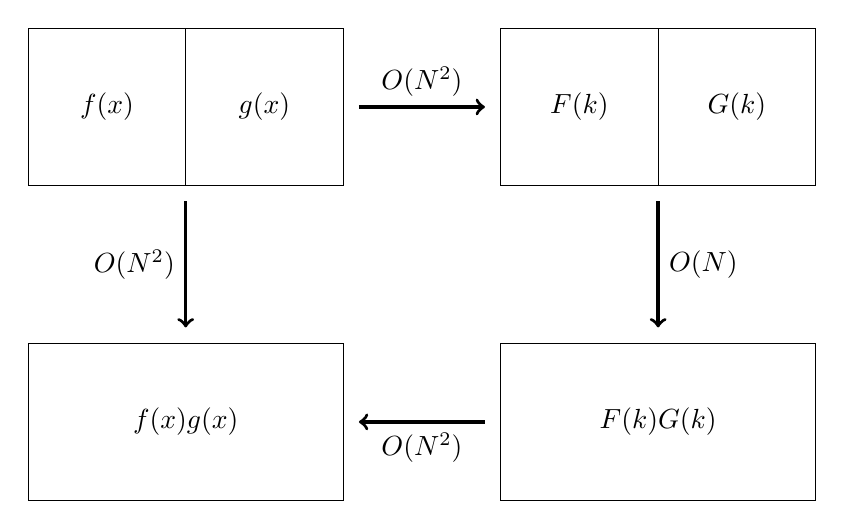
\begin{tikzpicture}
            \draw (0, 3) rectangle (2, 5);
            \draw (2, 3) rectangle (4, 5);
            \draw (0, -1) rectangle (4, 1);

            \draw (6, 3) rectangle (8, 5);
            \draw (8, 3) rectangle (10, 5);
            \draw (6, -1) rectangle (10, 1);

            \draw[->,very thick] (2, 2.8) -- node[anchor=east] { $O(N^2)$ } (2, 1.2);
            \draw[->,very thick] (8, 2.8) -- node[anchor=west] { $O(N)$ } (8, 1.2);
            \draw[->,very thick] (4.2, 4) -- node[anchor=south] { $O(N^2)$ } (5.8, 4);
            \draw[<-,very thick] (4.2, 0) -- node[anchor=north] { $O(N^2)$ } (5.8, 0);

            \node at (1, 4) { $f(x)$ };
            \node at (3, 4) { $g(x)$ };
            \node at (7, 4) { $F(k)$ };
            \node at (9, 4) { $G(k)$ };
            \node at (2, 0) { $f(x)g(x)$ };
            \node at (8, 0) { $F(k)G(k)$ };

        \end{tikzpicture}

    \end{figure}

\end{frame}

\begin{frame}[fragile]{Implementação da multiplicação indireta de polinômios}
    \inputsnippet{cpp}{34}{49}{codes/polynomial_dft.cpp}
\end{frame}

